\documentclass{standalone}
\usepackage{tikz}
\usepackage{ctex,siunitx,ninecolors}
\setCJKmainfont{Noto Serif CJK SC}
\usepackage{tkz-euclide}
\usepackage{amsmath}
\usetikzlibrary{patterns, calc}
\usetikzlibrary {decorations.pathmorphing, decorations.pathreplacing, decorations.shapes,}
\begin{document}
\small
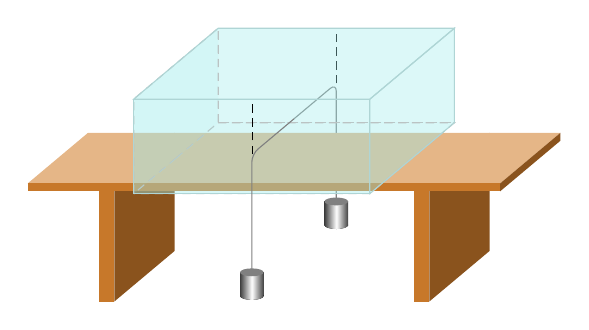
\begin{tikzpicture}[>=latex,scale=1.0]
  % \useasboundingbox(-1.4,-1.4)rectangle(1.4,1.4);
  \foreach \x[count=\i] in {40,220}
  {
    \coordinate (B\i) at ([shift=(\x:0.7)]0,-1);
    \fill[left color=darkgray,right color=darkgray,middle color=white]([yshift=-3mm]B\i)ellipse(0.15 and 0.05);
    \fill[left color=darkgray,right color=darkgray,middle color=white]([xshift=-1.5mm]B\i)rectangle++(0.3,-0.3);
    \fill[gray](B\i)ellipse(0.15 and 0.05);
  }
  \draw[gray,rounded corners=1mm](B1)--++(0,1.5)--++(220:0.7);
  \draw[ultra thin,densely dashed]([yshift=1.5cm]B1)--++(0,0.7);
  \foreach \x[count=\i] in {-2,2}
  {
    \coordinate (A\i) at ([shift=(220:0.5)]\x,0);
    \fill[brown6]([xshift=-0.1cm]A\i)rectangle++(0.2,-1.5);
    \fill[brown4]([xshift=0.1cm]A\i)--++(0,-1.5)--++(40:1.0)--++(0,1.5);
  }
  \fill[brown8](3,0)--++(40:0.5)--++(-6,0)--++(220:1.0)--++(6,0)--cycle;
  \fill[brown6]([shift=(220:0.5)]-3,0)--++(6,0)--++(0,-0.1)--++(-6,0)--cycle;
  \fill[brown4]([shift=(220:0.5)]3,0)--++(0,-0.1)--++(40:1.0)--++(0,0.1)--cycle;
  \draw[lightgray,fill=cyan9,fill opacity=0.4,densely dashed](-1.5,0)--++(40:0.7)--++(0,1.2)--++(220:1.4)--++(0,-1.2)--cycle;
  \draw[lightgray,fill=cyan9,fill opacity=0.3,densely dashed]([shift=(40:0.7)]-1.5,0)rectangle++(3,1.2);
  \draw[lightgray,fill=cyan9,fill opacity=0.35,densely dashed]([shift=(40:0.7)]-1.5,0)--++(3,0)--++(220:1.4)--++(-3,0);
  \draw[cyan9!50!lightgray,fill=cyan9,fill opacity=0.1]([shift=(220:0.7)]1.5,0)--++(40:1.4)--++(0,1.2)--++(220:1.4)--cycle;
  \draw[cyan9!50!lightgray,fill=cyan9,fill opacity=0.1]([shift=(220:0.7)]-1.5,0)rectangle++(3,1.2);
  \draw[cyan9!50!lightgray,fill=cyan9,fill opacity=0.1](-1.5,1.2)--++(40:0.7)--++(3,0)--++(220:1.4)--++(-3,0)--cycle;
  \draw[gray,rounded corners=1mm](B2)--++(0,1.5)--++(40:0.7);
  \draw[ultra thin,densely dashed]([yshift=1.5cm]B2)--++(0,0.7);
  % \fill[left color=darkgray,right color=darkgray]([xshift=])
\end{tikzpicture}
\end{document}